% Session 5 -- the three scenarios for one Fermi surface: metal, gapped SC, nodal SC.
% Placement: sec. "Three scenarios for one Fermi surface", after the enumerated list.
% Rendered by figures/blender/s05f02_fsgap.py, labels in figures/overlays/s05f02_fsgap.tex.
\begin{aqmfigure}{fig:s05:fsgap}{One Fermi surface with three outcomes. Each panel shows the
Brillouin zone with a small Fermi pocket around $\Gamma$, and the height of the tube standing on the
pocket is the minimum of the quasiparticle energy $E(\mathbf k)=\sqrt{\varepsilon(\mathbf
k)^2+|\Delta(\mathbf k)|^2}$ as we go once around it. Since $\varepsilon=0$ on the Fermi surface,
this minimum is $|\Delta|$ evaluated there, which is why the pairing function only matters \emph{on}
the Fermi surface. (a) Without pairing the whole pocket is at zero energy, which is a metal. (b) A
constant $\Delta_0$ lifts every point of it by the same amount, which gives a full gap. (c) The
$d$-wave gap (5.13) vanishes on the zone diagonals, the red lines, and the pocket crosses them in
four places, so four gapless points survive in a superconductor that is gapped everywhere else.
Nodes in other parts of the zone do not appear in the spectrum, and only nodes that intersect the
Fermi surface give gapless quasiparticles.}
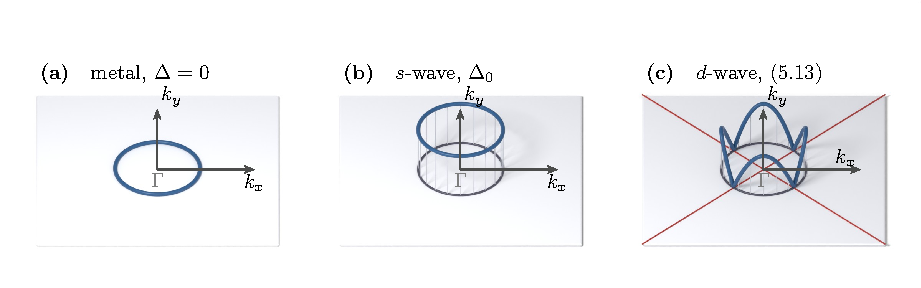
\includegraphics{figures/pdf/s05f02_fsgap.pdf}
\end{aqmfigure}
